
\section{Agregacja globalnych macierzy mas i sztywności}
\label{sec:agregacja}

Metoda agregacji macierzy globalnych zostanie przedstawiona na przykładzie macierzy sztywności dwóch elmentów kwadrratowych i obiektu z nich zbudowanego. Wspomniany obiekt przedstawia rysunek \ref{fig:agreg}. Czerne cyfry oznaczają numeracje lokalną wewnątrz elmentu, a czerwone numerację globalną.

Algorytm agregacji polega na umieszczaniu odpowiednich elementów macierzy lokalnych do macierzy globalnej. Pokrywające się elmenty są sumowane. Ponieważ podmacierz sztywności dla jednego punktu lub zależności pomiędzy punktami jest umieszczana w macierzy globalnej bez wewnętrznych zmian, przyjmijmy zapis uproszczony:

\begin{figure}[h]
\centering
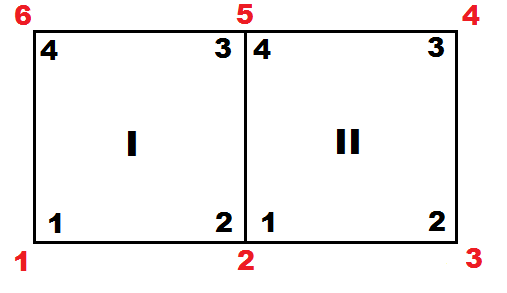
\includegraphics[width=10cm]{Zdjecia/3/agregacja}
\caption{Dwa elementy skończone kwadratowe tworzące obiekt}
\label{fig:agreg}
\end{figure}

\begin{gather}
	\textbf{K}_n^{ij} = \begin{bmatrix} 
	 	K^{ij}_{xx} & K^{ij}_{xy} \\
	 	K^{ij}_{xy} & K^{ij}_{yy} \\
	\end{bmatrix}
\end{gather}

gdzie
\begin{eqwhere}[2cm]
	\item[$i, j$] numery punktów
	\item[$n$] numer elementu
	\item[$x, y$] współrzędne punktów.
\end{eqwhere}

W takim wypadku lokalne macierze sztywności dla obydwu elementów możemy zapisać jako:

\begin{gather}
	\textbf{K}_{I} = \begin{bmatrix} 
	 	\textbf{K}^{11}_I & \textbf{K}^{12}_I & \textbf{K}^{13}_I & \textbf{K}^{14}_I \\
	 	\textbf{K}^{21}_I & \textbf{K}^{22}_I & \textbf{K}^{23}_I & \textbf{K}^{24}_I \\
	 	\textbf{K}^{31}_I & \textbf{K}^{32}_I & \textbf{K}^{33}_I & \textbf{K}^{34}_I \\
	 	\textbf{K}^{41}_I & \textbf{K}^{42}_I & \textbf{K}^{43}_I & \textbf{K}^{44}_I
	\end{bmatrix} \\
	\textbf{K}_{II} = \begin{bmatrix} 
	 	\textbf{K}^{11}_{II} & \textbf{K}^{12}_{II} & \textbf{K}^{13}_{II} & \textbf{K}^{14}_{II} \\
	 	\textbf{K}^{21}_{II} & \textbf{K}^{22}_{II} & \textbf{K}^{23}_{II} & \textbf{K}^{24}_{II} \\
	 	\textbf{K}^{31}_{II} & \textbf{K}^{32}_{II} & \textbf{K}^{33}_{II} & \textbf{K}^{34}_{II} \\
	 	\textbf{K}^{41}_{II} & \textbf{K}^{42}_{II} & \textbf{K}^{43}_{II} & \textbf{K}^{44}_{II}
	\end{bmatrix}.
\end{gather}

Macierze te mają wymiar 8x8, co odpowiada czterem punktom i dwóm współrzędnym dla każdego punktu. Macierz globalna wobec tego będzie miała wymiar 12x12 (6x6 podmacierzy). Poniżej przedstawione jest wyznaczanie kilku elmentów macierzy globalnej.

Dla globalnego punktu 1 mamy:
\begin{equation}
	\textbf{K}^{11} = \textbf{K}_I^{11},
\end{equation}
ponieważ punkt globalny 1 pokrywa się z punktem 1 macierzy I.

Dla globalnego punktu 2 mamy:
\begin{equation}
	\textbf{K}^{22} = \textbf{K}_I^{22} + \textbf{K}_{II}^{11},
\end{equation}
ponieważ punkt globalny 2 pokrywa się z punktem 2 macierzy I oraz punktem 1 macierzy II.

Dla zależności globalnych punktów 2 i 3 mamy:
\begin{equation}
	\textbf{K}^{23} = \textbf{K}_{II}^{12},
\end{equation}
ponieważ punkt globalny 2 pokrywa się z punktem 1, a punkt globalny 3 z punktem 2 macierzy II.

Dla zależności globalnych punktów 2 i 5 mamy:
\begin{equation}
	\textbf{K}^{25} = \textbf{K}_{I}^{23} + \textbf{K}_{II}^{14},
\end{equation}
ponieważ punkt globalny 2 pokrywa się z punktem 2 macierzy I oraz punktem 1 macierzy II, a punkt globalny 5 z punktem 3 macierzy I oraz punktem 4 macierzy II.

Uwzględniając że sztywność względna punktów nie będących ze sobą w sąsiedztwie (np. 1 i 3 w I) wynosi 0, macierz globalna przyjmuje postać:

\begin{gather}
	\textbf{K} = \begin{bmatrix} 
	 	\textbf{K}^{11}_I & \textbf{K}^{12}_I & 0 & 0 & 0 & \textbf{K}^{14}_I  \\
	 	\textbf{K}^{21}_I & \textbf{K}^{22}_I + \textbf{K}^{11}_{II}  & \textbf{K}^{12}_{II} & 0 & \textbf{K}_{I}^{23} + \textbf{K}_{II}^{14} & 0 \\
	 	0 & \textbf{K}^{21}_{II} & \textbf{K}^{22}_{II} & \textbf{K}^{23}_{II} & 0 & 0 \\
	 	0 & 0 & \textbf{K}^{32}_{II} & \textbf{K}^{33}_{II} & \textbf{K}^{34}_{II} & 0 \\
		0 & \textbf{K}_{I}^{32} + \textbf{K}_{II}^{41} & 0 & \textbf{K}^{43}_{II} & \textbf{K}^{33}_{I} + \textbf{K}	^{44}_{II} & \textbf{K}^{34}_{I} \\
		\textbf{K}^{41}_I & 0 & 0 & 0 & \textbf{K}^{43}_I & \textbf{K}^{44}_I.
	\end{bmatrix}
\end{gather}

Oczywistym jest, że w przypadku innej numeracji węzłów globalnych zmieni się układ macierzy globalnej. Nie ma to jednak wpływu na ostateczny wynik rozwiązania MES. W modelach o dużej liczbie elmentów skończonych macierze mas i sztywności są macierzami rzadkimi. Wykorzystuje się to w obliczeniach do oszczędzania pamięci komputera, poprzez zapis w pamięci tylko wartości niezerowych oraz ich położenia w macierzy. 

Macierz mas wyznaczona w przedstawiony sposób jest nazywana macierzą konsystentną. Często stosuje się macierze skupione, które zawierają elementy tylko na diagonali. Pozwala to bardzo przyspieszyć obliczenia. Takie rozwiązanie jest ściśle rzecz biorąc niepoprawne, ponieważ nie ma algorytmu, który pozwala obliczyć macierz skupioną i zachować w pełni właściwości modelu. Macierze skupione oblicza się np. poprzez sumowanie wszystkich elmentów w wierszu i umieszczanie tej sumy na elemencie diagonalnym. Dobrą stroną macierzy skupionych jest fakt, że rozwiązanie pozostaje zbieżne.



















